\documentclass[12pt,titlepage,a4paper]{report}

% Texte
\usepackage[utf8]{inputenc}
\usepackage[T1]{fontenc}
\usepackage[french]{babel}
\usepackage[babel=true]{csquotes}
\usepackage{lmodern}
\usepackage{minted}
\usemintedstyle{trac}

% Numéroter les chapitres a partir de chaque début de partie
\makeatletter\@addtoreset{chapter}{part}\makeatother

% Mise en page
\usepackage{url}
\usepackage[top=2.1cm,bottom=2cm,left=1cm,right=1cm]{geometry}
\usepackage{hyperref}
\hypersetup{
    colorlinks=false,
    pdfborder={0 0 0},
}
\usepackage{multirow}

% TOC
\usepackage[french]{minitoc}
\setcounter{tocdepth}{2}
\setcounter{minitocdepth}{3}
\setlength{\mtcindent}{0pt}

% Images
\usepackage{float}
\usepackage{wrapfig}
\usepackage{graphicx}
% Pour inclure des pages PDF
\usepackage[final]{pdfpages}

% Couverture
\usepackage{templateINSA}
\initINSA

% Citations
\usepackage{epigraph}
\setlength\epigraphwidth{12cm}
\setlength\epigraphrule{0pt}

\usepackage{etoolbox}

\makeatletter
\patchcmd{\epigraph}{\@epitext{#1}}{\itshape\@epitext{#1}}{}{}
\makeatother

\usepackage[nottoc, notlof, notlot]{tocbibind}

\title{Segmentation d'image à l'aide de statistiques et d'information spatiales}
\author{Manon \bsc{Ansart}\\Antoine \bsc{Augusti}}

\renewcommand\soustitre{Analyse d'article scientifique}
\renewcommand\infoBig{TIM}
\renewcommand\infoSmall{ASI4 2014-2015}
\newcommand\bddGraphe{base de données orientée graphe}

\def\changemargin#1#2{\list{}{\rightmargin#2\leftmargin#1}\item[]}
\let\endchangemargin=\endlist

%% -- Document
\begin{document}
	\titleINSA{15}{images/lena.png}{0}{0}{300}{}{}
	\dominitoc
	\tableofcontents

	\chapter{Introduction}
	\minitoc
		\section{Objectifs}
			Le but de ce projet est de comprendre un article de recherche du domaine du traitement d'images. L'article que nous devons étudier s'intitule \enquote{\textit{A quad-tree approach to image segmentation which combines statistical and spatial information}} écrit par M. Spann et R. Wilson en 1984. Après l'étude de cet article, nous devons produire un rapport expliquant ce que nous avons compris de celui-ci. Une présentation orale est également prévue.
		
		\section{Définitions préliminaires}
			Afin d'étudier dans de bonnes conditions notre article scientifique, il est nécessaire de définir certains termes qui seront utilisés dans la suite du présent rapport.

\subsection{La segmentation d'image}
	\enquote{La segmentation d'image est une opération de traitement d'images qui a pour but de rassembler des pixels entre eux suivant des critères pré-définis. Les pixels sont ainsi regroupés en régions, qui constituent un pavage ou une partition de l'image.}\cite{wikiSegmentationImage} On peut par exemple vouloir distinguer des objets du fond de l'image. Le terme de \enquote{binarisation} est utilisé quand on sépare une image en deux classes.\\

	La segmentation d'image est un des thèmes les plus courants en traitement d'images aujourd'hui car la mise au point d'algorithmes de segmentation de haut niveau reste un véritable challenge. À ce jour, les principales méthodes de segmentation sont au nombre de quatre :
	\vspace{10px}
	\begin{enumerate}
		\item Segmentation fondée sur les régions (\textit{region-based segmentation}). On y retrouve deux méthodes : la croissance de région (\textit{region-growing}) et la décomposition / fusion (\textit{split and merge}).
		\item Segmentation fondée sur les contours (\textit{edge-based segmentation}) ;
		\item Segmentation par classification (\textit{classification}) ou par le seuillage des pixels en fonction de leur intensité (\textit{thresholding}) ;
		\item Segmentation fondée par une utilisation commune des trois premières segmentations.
	\end{enumerate}

		\section{Le quadtree}
			De manière générale, un quadtree est une structure de données de type arbre dans laquelle chaque nœud possède quatre fils. Dans notre cas, on utilise un quadtree dit \enquote{région} qui représente l'image en deux dimensions, en décomposant la région en quatre parties égales, puis chaque partie en quatre sous-parties et ainsi de suite. Chaque nœud du quadtree représente un pixel noir, blanc ou gris. Un nœud gris contient un mélange de pixels blanc et noirs. On obtient un quadtree complet quand on subdivise l'image de manière récursive de manière à ce que le quadtree ne contienne que des nœuds de pixels blancs ou noirs.\\

Un quadtree \enquote{région} ayant une profondeur $n$ peut être utilisé pour représenter une image de $2^{n}\times2^{n}$ pixels, où la valeur de chaque pixel est 0 (noir) ou 1 (blanc). Des exemples de quadtree sont représentés dans les figures \ref{fig:quadtree} et \ref{fig:quadtree2}.

\begin{figure}[H]
	\centering
	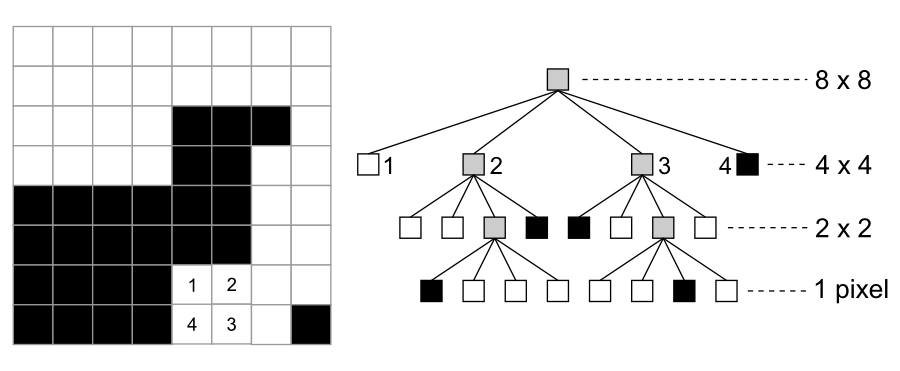
\includegraphics[scale=0.8]{images/quadtree.png}
	\caption{Représentation d'un quadtree.}
	\label{fig:quadtree}
\end{figure}

\begin{figure}[H]
	\centering
	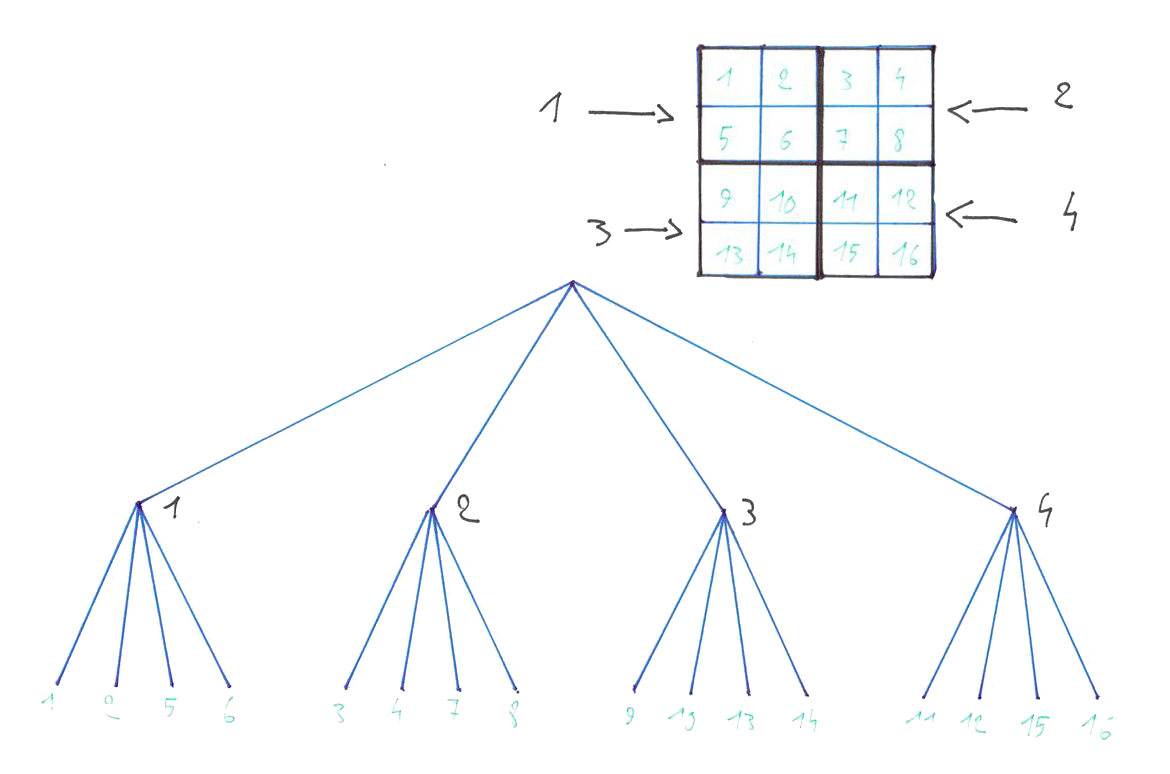
\includegraphics[scale=0.4]{images/quadtree-dessin.jpg}
	\caption{Représentation d'un quadtree.}
	\label{fig:quadtree2}
\end{figure}

Le passage d'un niveau $k$ au niveau $k + 1$ est représenté dans la figure \ref{fig:quadtree-niveaux}. Plus la valeur d'un niveau est élevée plus l'image est petite.

\begin{figure}[H]
	\centering
	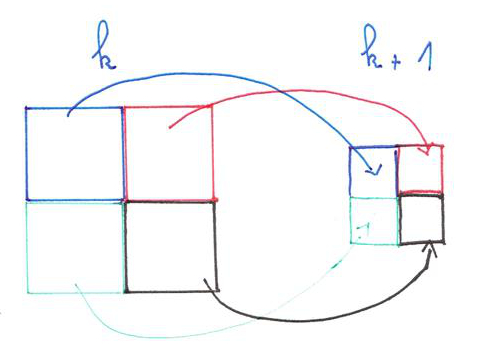
\includegraphics[scale=0.6]{images/quadtree-niveaux.jpg}
	\caption{Représentation du passage d'un niveau à un autre d'un quadtree.}
	\label{fig:quadtree-niveaux}
\end{figure}

	%% -- Bibliographie
	\bibliographystyle{plain}
	\bibliography{bib}

\end{document}